\section{What moves the euro: the rates channel and the risk channel}\label{sec:euro}

On a G10 FX desk, the euro is driven first by rates.
Two channels link euro-area rates to the exchange rate.
In the \emph{rates channel}, a rise of euro rates relative to foreign rates makes euro assets more attractive and raises the euro; it also changes the forward points through covered interest parity.
In the \emph{risk channel}, doubts about the sustainability of the debt of a member state widen its sovereign spread over the German Bund, a risk premium appears on the euro and the euro falls, especially against the Swiss franc, the European safe haven.
This section measures both channels with public data.
It prepares the hedging problem of Section~\ref{sec:hedging}: a euro-based investor needs to know when the euro is likely to fall.

\subsection{Specification}

The variables are monthly changes of monthly averages (Decision~D18).
The dependent variable is the percentage change of the monthly average of EURUSD or EURCHF, positive when the euro appreciates.
The rates channel is measured by the change in the 3-month rate differential, $\Delta(i_{\mathrm{EUR}} - i_{\mathrm{USD}})$ or $\Delta(i_{\mathrm{EUR}} - i_{\mathrm{CHF}})$, and by the change in the 10-year differential between the Bund and the US Treasury.
The risk channel is measured by the change in the 10-year spreads of Italy (BTP) and France (OAT) over the Bund.
Rates, spreads and their changes are in percentage points.
Each regression
\begin{equation}\label{eq:euro-reg}
  \Delta s_t = \alpha + \beta_{\mathrm{rates}}\, \Delta(\text{rate differential})_t + \beta_{\mathrm{risk}}\, \Delta(\text{spread})_t + \varepsilon_t
\end{equation}
is estimated by ordinary least squares with Newey--West standard errors \citep{newey1987}, which remain valid when the residuals are heteroskedastic or autocorrelated; the latter is expected here because averaging daily data over a month induces autocorrelation in monthly changes.
The coefficients are contemporaneous associations, not causal effects: both sides react to the same news within the month.

\subsection{Results}

\begin{table}[h]
\centering
\footnotesize
\begin{tabular}{@{}lrrrr@{}}
\toprule
 & (1) EURUSD & (2) EURUSD & (3) EURCHF & (4) EURCHF ex-floor \\
\midrule
$\Delta(i_{\mathrm{EUR}} - i_{\mathrm{USD}})$, 3M & 1.08 & 0.20 &  &  \\
 & (1.1) & (0.2) &  &  \\[2pt]
$\Delta(i_{\mathrm{EUR}} - i_{\mathrm{CHF}})$, 3M &  &  & -1.00 & -0.33 \\
 &  &  & (-1.0) & (-0.5) \\[2pt]
$\Delta(y_{\mathrm{Bund}} - y_{\mathrm{UST}})$, 10Y &  & 5.76 &  &  \\
 &  & (5.1) &  &  \\[2pt]
$\Delta$ BTP--Bund, 10Y & -2.27 & -2.65 & -0.65 & -2.33 \\
 & (-4.1) & (-4.3) & (-1.0) & (-3.3) \\[2pt]
$\Delta$ OAT--Bund, 10Y &  & 1.07 &  &  \\
 &  & (0.5) &  &  \\[2pt]
Constant & 0.03 & 0.04 & -0.15 & -0.16 \\
 & (0.2) & (0.3) & (-2.1) & (-2.1) \\[2pt]
\midrule
$R^2$ & 0.05 & 0.16 & 0.02 & 0.09 \\
Months & 329 & 329 & 325 & 284 \\
\bottomrule
\end{tabular}

\caption{Regressions of the monthly percentage change of the euro on the changes in rate differentials and sovereign spreads (percentage points), February 1999 -- August 2026. $t$-statistics with Newey--West standard errors (5 lags) in parentheses. Column (4) excludes the period of the Swiss National Bank floor on EURCHF (September 2011 -- January 2015). Generated by \texttt{scripts/euro\_drivers.py}.}
\label{tab:euro}
\end{table}

\paragraph{The risk channel is significant against both currencies.}
In column (1), a widening of the BTP--Bund spread by 10 basis points is associated with a fall of the euro against the dollar of about 0.23\% in the same month ($t = -4.1$).
The effect survives the addition of the 10-year rate differential and of the French spread in column (2).
Against the Swiss franc, the full-sample estimate in column (3) is small and not significant, but this is an artefact of the Swiss National Bank floor: from September 2011 to January 2015 the franc was capped at 1.20 per euro, precisely during the euro-area debt crisis, so EURCHF could not respond to euro risk.
Without these months, in column (4), the coefficient is $-2.33$ ($t = -3.3$), the same order of magnitude as against the dollar.
The negative constant of the EURCHF regressions, $-0.15\%$ a month, is the trend appreciation of the franc against the euro over the sample, about 1.8\% a year.

\paragraph{The rates channel works through long rates.}
The change in the 3-month differential is not significant in any column, whereas the change in the 10-year differential between the Bund and the US Treasury is the strongest variable of column (2): a 10-basis-point rise of the Bund relative to the Treasury goes with a rise of the euro of about 0.58\% ($t = 5.1$).
Two reasons explain the difference.
First, short rates move with policy decisions, which are largely anticipated; the exchange rate reacts to changes in the expected path of policy, which long rates capture.
Second, monthly averages of short rates are smooth, so their changes contain little news.
The French spread adds no information once the Italian spread is in the regression.

\paragraph{The risk channel is not constant.}
Figure~\ref{fig:euro-beta} reports the coefficient on the BTP--Bund spread over rolling 36-month windows.
Before 2008 it is erratic, because sovereign spreads were a few tens of basis points and barely moved, so the coefficient is poorly identified.
Against the dollar it reached about $-1\%$ per 10 basis points at the height of the debt crisis in 2011, and it has been negative since 2018, between about $-0.1\%$ and $-0.7\%$; against the franc it has been of similar size since 2018.
In between, for windows ending in 2016--2018, it turned positive, a period dominated by the asset purchases of the ECB, which lowered both the euro and Italian spreads; this is consistent with the two channels pulling in opposite directions when the central bank itself drives the spread.

\begin{figure}[h]
\centering
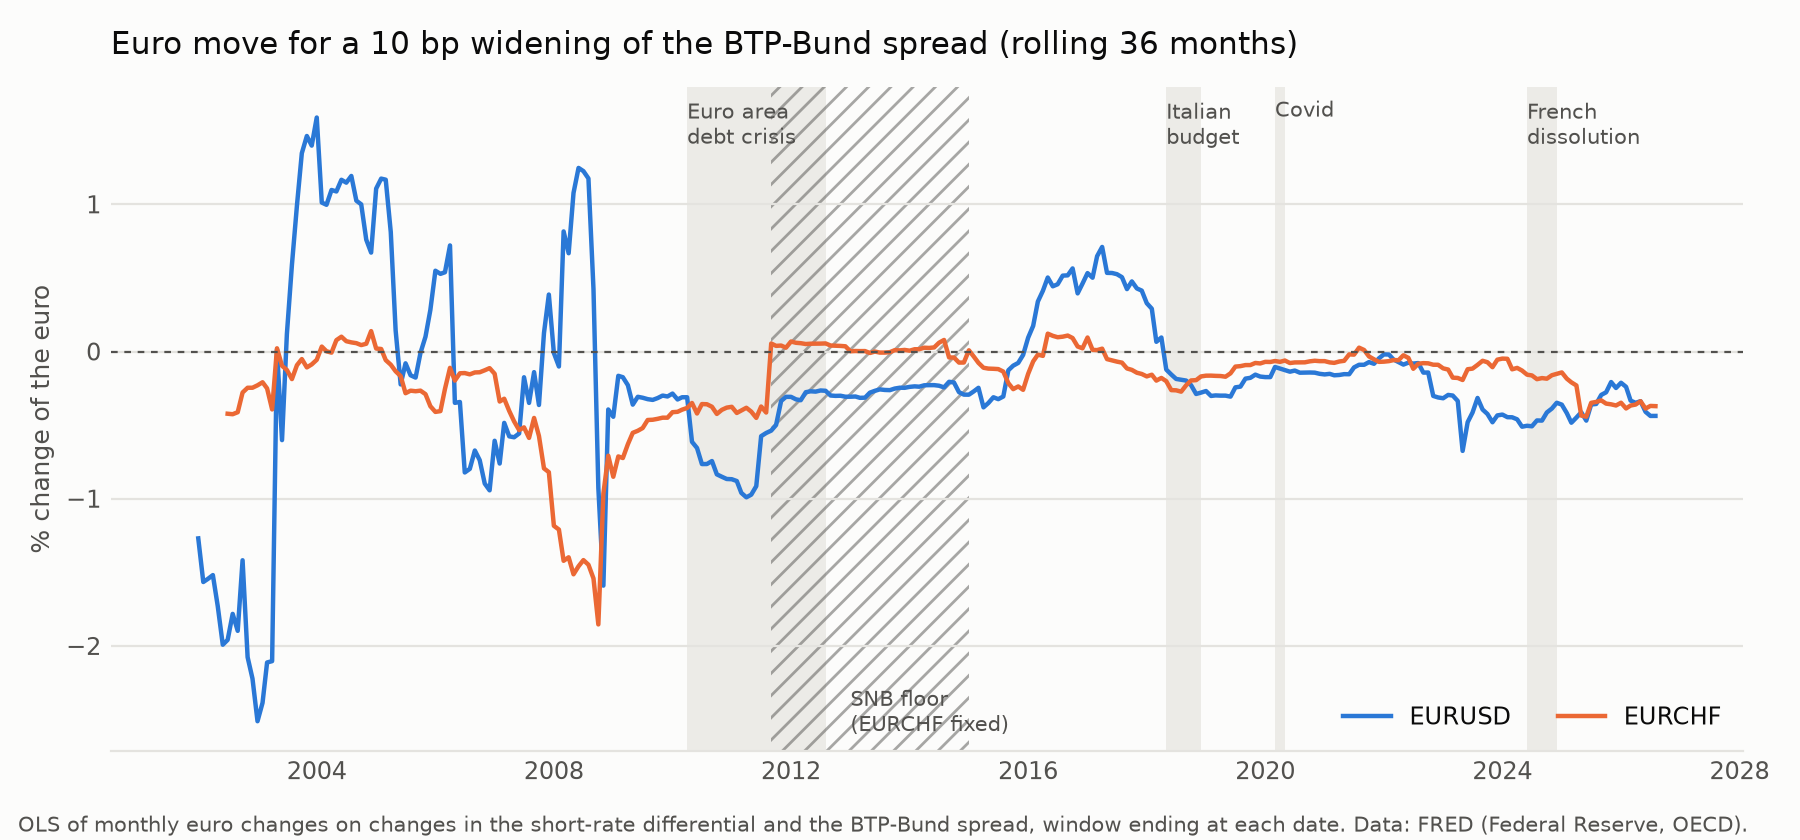
\includegraphics[width=\textwidth]{figures/euro_risk_beta.png}
\caption{Coefficient on the change in the BTP--Bund spread in regressions of the monthly change of EURUSD and EURCHF on the short-rate differential and the spread, over rolling 36-month windows ending at each date, scaled to a 10-basis-point widening. Hatched: Swiss National Bank floor. Generated by \texttt{scripts/euro\_drivers.py}.}
\label{fig:euro-beta}
\end{figure}

\subsection{What is left out, and why}

A trader would also follow ECB meetings, sovereign debt auctions and the carry and roll-down of bonds.
These are monitoring and rates-desk topics rather than questions that public data can answer for 27 years; they are left out of the project, for the reasons given in Decision~D19.
